\documentclass[letterpaper]{scrreprt}

%% Language and font encodings
\usepackage[spanish]{babel}
\usepackage[utf8]{inputenc}
\usepackage[T1]{fontenc}
\usepackage{subcaption}

\usepackage{pdfpages}
\usepackage{float}
%% Sets page size and margins
\usepackage[letterpaper,top=3cm,bottom=2cm,left=3cm,right=3cm,marginparwidth=1.75cm]{geometry}

%% Useful packages
\usepackage{amsmath}
\usepackage{graphicx}
\usepackage[colorinlistoftodos]{todonotes}
\usepackage[colorlinks=true, allcolors=black]{hyperref}

\usepackage{geometry}
\usepackage{xcolor}
\definecolor{titlepagecolor}{cmyk}{0,.1098,.8118,0}
\definecolor{namecolor}{cmyk}{.6,.3,0,0.98} % Here
\setlength{\parindent}{4em}
\setlength{\parskip}{1em}
\renewcommand{\baselinestretch}{1.5}

\title{LEGO Package Verifier}
\subtitle{Documento de Diseño}
\author{Nicolás Camacho Plazas, Mateo Florido Sanchez}


\graphicspath{{Figures/}}

\begin{document}
% ----------------------------------------------------------------
\begin{titlepage}
	\newgeometry{left=7.5cm}
	\pagecolor{titlepagecolor}
	\noindent
	
\includegraphics[width=4cm]{Extras/javeriana.png}\\[-1em]
	\color{namecolor}
	\makebox[0pt][l]{\rule{1.3\textwidth}{1.5pt}}
	\par
	\noindent
	\textbf{\LARGE \textsf{LEGO Package Verifier - Documento Entrega Final}}
	\vfill
	\noindent
	{\huge \textsf{Versión 1.0}}
	\vskip\baselineskip
	\noindent
	\textsf{Febrero 2020}
\end{titlepage}
\restoregeometry % restores the geometry
\nopagecolor% Use this to restore the color pages to white
% ----------------------------------------------------------------

\maketitle
\noindent
Documento Entrega Final\\ 
Versión v2.0, Junio 2020\\
Authors - Nicolás Camacho Plazas, Mateo Florido\\
This entire document is licensed under GNU General Public License v3.0. Permissions of this strong copyleft license are conditioned on making available complete source code of licensed works and modifications, which include larger works using a licensed work, under the same license. Copyright and license notices must be preserved. Contributors provide an express grant of patent rights.\\
LEGO System A/S, DK-7190 Billund, Denmark. LEGO, the LEGO logo, the Minifigure, DUPLO, LEGENDS OF CHIMA, NINJAGO, BIONICLE, MINDSTORMS and MIXELS are trademarks and copyrights of the LEGO Group. ©2019 The LEGO Group. All rights reserved.

\newpage

\tableofcontents

% ______________________
% Cap. Definición de Problema
% Solucion a proponer, Alcance, Requerimientos técnicos y tecnologicos.
% ______________________

\chapter{Alcance}
El alcance de nuestro producto estará orientado a intentar reconocer las diferentes piezas de un set. Sin embargo, se ha decidido dividir los alcances en diferentes categorías que se presentarán a continuación.

\section{Entradas}
Las entradas estarán dadas por un set de máximo 8 tipos de piezas sin importar su color. Las piezas que pueden ser reconocidas son:

\begin{figure}[H]
	\begin{subfigure}{0.5\textwidth}
		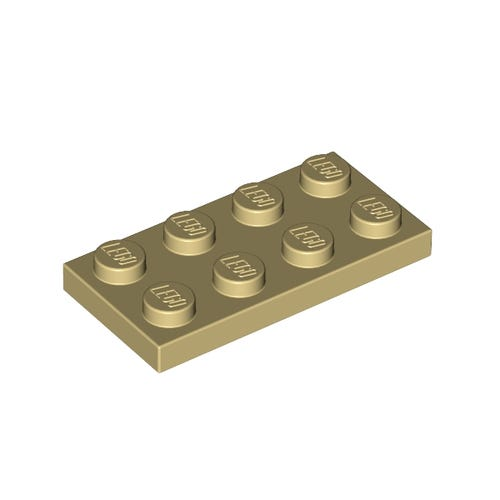
\includegraphics[width=0.9\linewidth, height=5cm]{Bricks/plate2x4.jpeg} 
		\caption{Plate 2x4}
		\label{fig:subim1}
	\end{subfigure}
	\begin{subfigure}{0.5\textwidth}
		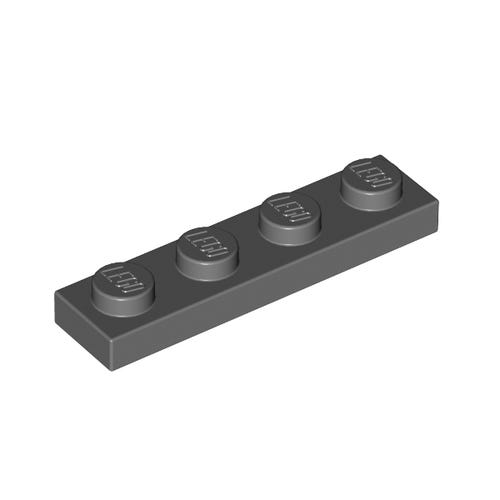
\includegraphics[width=0.9\linewidth, height=5cm]{Bricks/plate1x4.jpeg}
		\caption{Plate 1x4}
		\label{fig:subim2}
	\end{subfigure}
	\begin{subfigure}{0.5\textwidth}
		\centering
		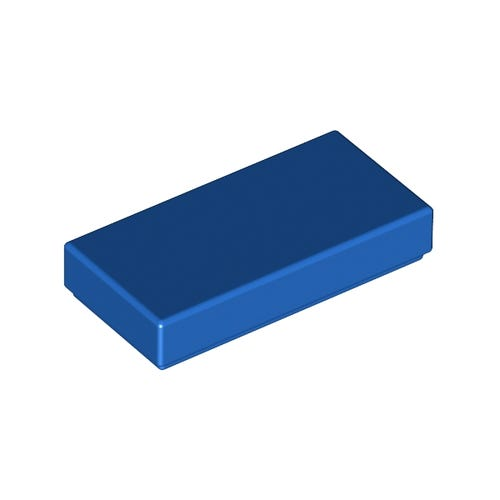
\includegraphics[width=0.4\linewidth, height=3cm]{Bricks/flattile1x2.jpeg}
		\caption{Flat Tile 1x2}
		\label{fig:subim3}
	\end{subfigure}
	\begin{subfigure}{0.5\textwidth}
		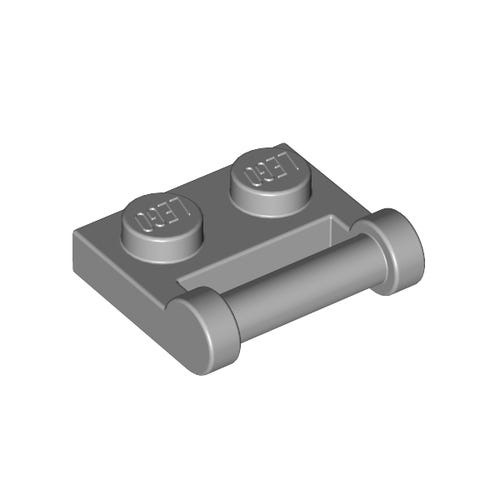
\includegraphics[width=0.9\linewidth, height=5cm]{Bricks/stick1x2.jpeg}
		\caption{Plate 1x2 W. Stick 3.18}
		\label{fig:subim3}
	\end{subfigure}
	\begin{subfigure}{0.5\textwidth}
		\centering
		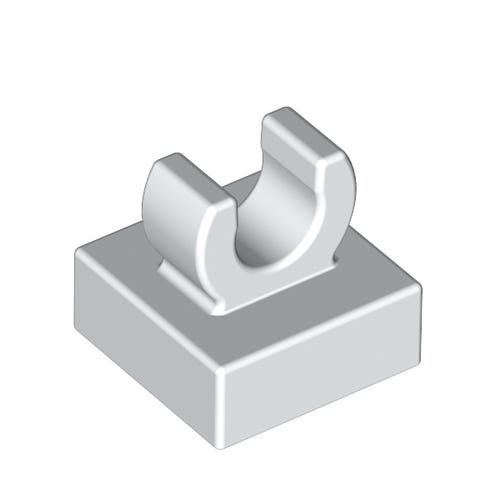
\includegraphics[width=0.4\linewidth, height=3cm]{Bricks/1x1up.jpeg}
		\caption{Plate 1x1 W. Up Right Holder}
		\label{fig:subim3}
	\end{subfigure}
	\begin{subfigure}{0.5\textwidth}
		\centering
		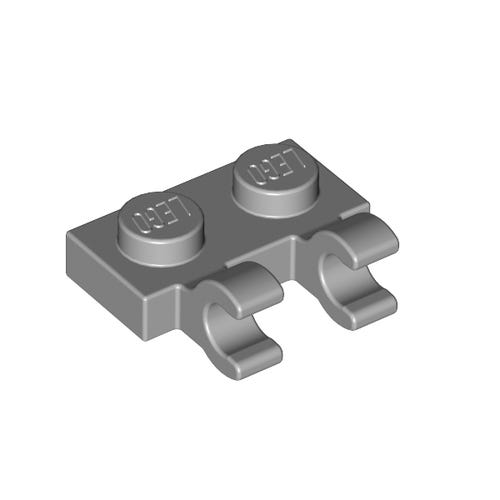
\includegraphics[width=0.4\linewidth, height=3cm]{Bricks/1x2holder.jpeg}
		\caption{Plate 1x2 W. Holder Vertical}
		\label{fig:subim3}
	\end{subfigure}
	\begin{subfigure}{0.5\textwidth}
		\centering
		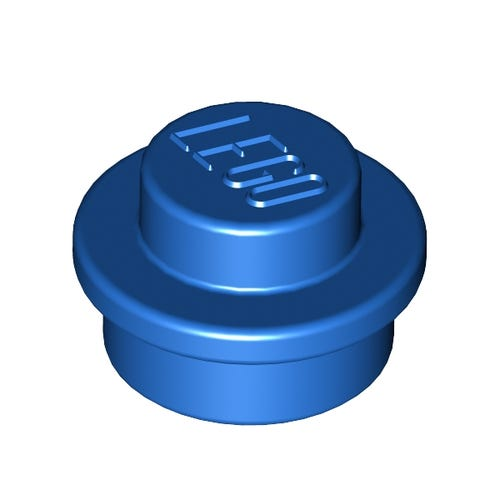
\includegraphics[width=0.4\linewidth, height=3cm]{Bricks/round1x1.jpeg}
		\caption{Round Plate 1x1}
		\label{fig:subim3}
	\end{subfigure}
	\begin{subfigure}{0.5\textwidth}
		\centering
		
\includegraphics[width=0.4\linewidth, height=4cm]{Bricks/astronaut.jpg}
		\caption{miniFigure Astronaut Series 1}
		\label{fig:subim3}
	\end{subfigure}
	\caption{Piezas reconocibles}
	\label{fig:image2}
\end{figure}

\subsection{Entorno de Captura}
Estas piezas en un inicio entrarán al sistema mediante una captura de imagen a la banda transportadora donde se encuentran. 
\subsection{Iluminación}
Debe tener una iluminación uniforme en toda la captura para mitigar los errores. Se deben capturar las imágenes sin sombras o brillos que puedan entorpecer el reconocimiento de las piezas.
\subsection{Cámara}
La cámara debe de ubicarse a una altura constante que permita evitar el cambio del tamaño relativo de las piezas capturadas.
\subsection{Fondo}
Para realizar de forma más precisa el reconocimiento de las piezas, se debe utilizar un fondo uniforme de color negro de preferencia textura mate para evitar la refelexión de la luz.
\section{Salida}
Se obtiene una imágen en la que se encuentran bordeadas las piezas reconocidas con un contorno verde, además del número de pieza oficial de LEGO.

% ______________________
% Cap. Proceso
% ______________________

\chapter{Proceso}

Para el procesamiento de las piezas capturadas realizamos primero un downsample de la imagen mediante el uso de una pirámide Gaussiana (se usó pyrDown en OpenCV). Esto con el fin de reducir la resolución de la imagen a la mitad y evitar que se detecten multiples detalles no relevantes de nuestra imagen.

Luego, se realiza un desenfoque gaussiano con un kernel 5x5 sobre todo la imagen para facilitar la detección de las piezas. Debido a que el algoritmo de detección de bordes es sensible a la presencia de ruido de la imagen, se debe utilizar el desenfoque gaussiano mencionado anteriormente que mejora los resultados del algoritmo de detección.

Acorde a que las piezas tienen una forma definida y lo suficientemente diferente de otras, se binariza la imagen con el Método de Otsu para encontrar el umbral óptimo de la imagen. Con esto, podemos extraer la forma definida y realizar un reconocimiento de las diferentes propiedades que contiene cada pieza (número de lados, perímetro relativo y área relativa).

Con la imagen binarizada, se extraen los contornos de la imagen. Debido a que el algoritmo entrega todos los contornos posibles, solamente nos quedamos con los contornos externos de cada pieza de LEGO. Esto con el fin de no detectar otras características que no son relevantes. Finalmente, se aproximan los contornos usando solo sun puntos extremos; es decir, si tenemos un rectángulo, este será definido por 4 puntos.

En el tratamiento de cada contorno para detectar las piezas se evalúa si el contorno tiene un perímtero considerable. Esto se realiza para eliminar rastros de la imagen que pudieron quedar identificados. A continuación se aproximan los polígonos extraídos de los contornos con otro polígono con menos vértices esto con el fin de dejar la cantidad real de lados que contienen los contornos y dejar a un lado lados que pudieron ser identificados erróneamente. Para este método se utiliza el algoritmo Ramer-Douglas-Peucker (RDP).

Ya con el polígono aproximado, se obtienen las propiedades de número de lados, perímetro relativo y área relativa. Mediante las mediciones realizadas, se clasifican todas las piezas con los parámetros establecidos.

Finalmente, se escribe una imagen en la que se observan todas las piezas identificadas con su identificador único de LEGO y la palabra APPROVED o FAIL en caso de que se verificara la integridad del paquete analizado.



%\todo[inline, color=green!40]{This is an inline comment.}

%\bibliographystyle{alpha}
%\bibliography{sample}

\end{document}